\documentclass[border=10pt]{standalone}
\usepackage[svgnames]{xcolor}
\usepackage{amsmath}
\usepackage{pgfplots}
\pgfplotsset{compat=newest}
\usepackage[sfdefault]{FiraSans}
\usepackage{FiraMono}
\renewcommand*\familydefault{\sfdefault}
\begin{document}
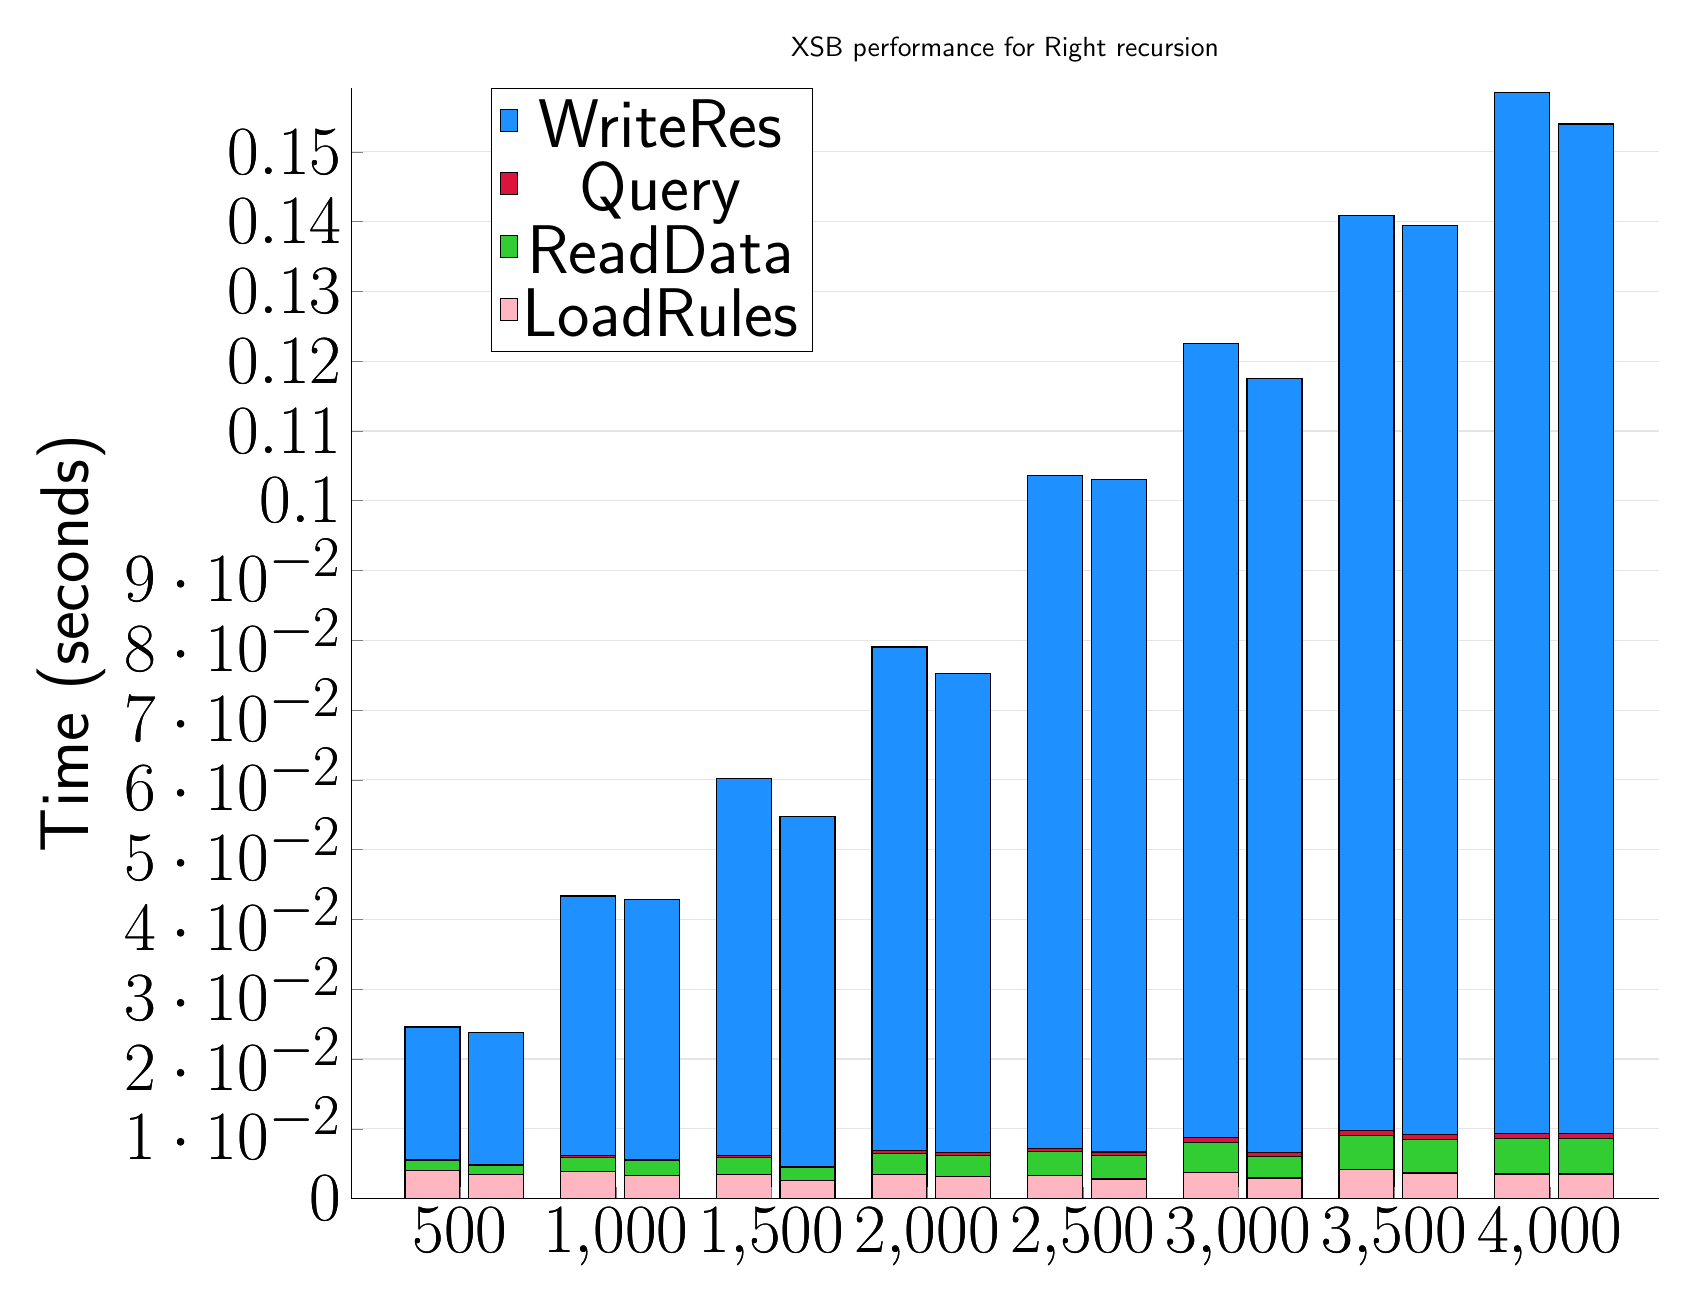
\begin{tikzpicture}
\begin{axis}[
   ybar stacked,
   title={XSB performance for Right recursion},
   bar shift=-10pt,
   width=1.5\textwidth,
   bar width=0.7cm,
   ymajorgrids, tick align=inside,
   major grid style={draw=gray!20},
   xtick=data,
   ymin=0, ymax=0.15917342821757002,
   axis x line*=bottom,
   axis y line*=left,
   enlarge x limits=0.1,
   legend style={
       at={(0.23, 1)},
       anchor=north,
       legend columns=1,
       font=\Huge,
   },
   ylabel={Time (seconds)},
   label style={font=\Huge},
   tick label style={font=\Huge},
]
\addlegendimage{fill=DodgerBlue, draw=black, line width=0.2pt}
\addlegendentry{WriteRes}
\addlegendimage{fill=Crimson, draw=black, line width=0.2pt}
\addlegendentry{Query}
\addlegendimage{fill=LimeGreen, draw=black, line width=0.2pt}
\addlegendentry{ReadData}
\addlegendimage{fill=LightPink, draw=black, line width=0.2pt}
\addlegendentry{LoadRules}
\addplot +[fill=LightPink, draw=black, line width=0.5pt] coordinates {
    (500, 0.003985087076822917)
    (1000, 0.0038352807362874333)
    (1500, 0.003471692403157553)
    (2000, 0.00342893600463867)
    (2500, 0.003315051396687823)
    (3000, 0.003738323847452797)
    (3500, 0.00418734550476074)
    (4000, 0.003536701202392577)
};
\addplot +[fill=LimeGreen, draw=black, line width=0.5pt] coordinates {
    (500, 0.0014839172363281267)
    (1000, 0.0020906925201416)
    (1500, 0.002444664637247724)
    (2000, 0.003040949503580727)
    (2500, 0.0034172534942626966)
    (3000, 0.0042877197265625)
    (3500, 0.004839658737182614)
    (4000, 0.005053043365478513)
};
\addplot +[fill=Crimson, draw=black, line width=0.5pt] coordinates {
    (500, 0.00014098485310872364)
    (1000, 0.00021831194559733067)
    (1500, 0.00029198328653971334)
    (2000, 0.00043543179829915363)
    (2500, 0.000473340352376302)
    (3000, 0.0007103284200032554)
    (3500, 0.0007417201995849609)
    (4000, 0.0007369518280029297)
};
\addplot +[fill=DodgerBlue, draw=black, line width=0.5pt] coordinates {
    (500, 0.01897239685058594)
    (1000, 0.0371983846028646)
    (1500, 0.05398758252461752)
    (2000, 0.0721565882364909)
    (2500, 0.09641027450561511)
    (3000, 0.11377374331156408)
    (3500, 0.1311142444610597)
    (4000, 0.14914870262146007)
};
\end{axis}
\begin{axis}[
   ybar stacked,
   bar shift=13pt,
   width=1.5\textwidth,
   bar width=0.7cm,
   ymajorgrids, tick align=inside,
   major grid style={draw=none},
   xtick=data,
   ymin=0, ymax=0.15917342821757002,
   axis x line*=none,
   axis y line*=none,
   enlarge x limits=0.1,
   label style={font=\Huge},
   tick label style={font=\Huge},
]
\addplot +[fill=LightPink, draw=black, line width=0.5pt] coordinates {
    (500, 0.0034230000000000003)
    (1000, 0.0033439999999999998)
    (1500, 0.0025943333333333335)
    (2000, 0.003172333333333333)
    (2500, 0.0027816666666666667)
    (3000, 0.0029416666666666666)
    (3500, 0.00364566666666667)
    (4000, 0.0035303333333333332)
};
\addplot +[fill=LimeGreen, draw=black, line width=0.5pt] coordinates {
    (500, 0.0012956666666666674)
    (1000, 0.0020723333333333336)
    (1500, 0.001815)
    (2000, 0.0030310000000000003)
    (2500, 0.003395666666666663)
    (3000, 0.003058333333333333)
    (3500, 0.004817666666666667)
    (4000, 0.005053666666666667)
};
\addplot +[fill=Crimson, draw=black, line width=0.5pt] coordinates {
    (500, 0.0001193333333333323)
    (1000, 0.00021800000000000066)
    (1500, 0.000213999999999999)
    (2000, 0.0004353333333333293)
    (2500, 0.00047300000000000234)
    (3000, 0.000616666666666666)
    (3500, 0.000714666666666669)
    (4000, 0.0007363333333333342)
};
\addplot +[fill=DodgerBlue, draw=black, line width=0.5pt] coordinates {
    (500, 0.018995)
    (1000, 0.037186)
    (1500, 0.05008933333333334)
    (2000, 0.06862366666666667)
    (2500, 0.09641466666666666)
    (3000, 0.11093966666666666)
    (3500, 0.1302576666666667)
    (4000, 0.14466066666666666)
};
\end{axis}
\end{tikzpicture}

\end{document}
